\documentclass{article}
%\usepackage[utf8]{inputenc}
\usepackage[UTF8]{ctex}
\usepackage{xcolor}
\usepackage[colorlinks,linkcolor=blue,anchorcolor=blue,citecolor=blue]{hyperref}
\usepackage{subfigure}
\usepackage{geometry}
\usepackage{algorithm}  
\usepackage{algorithmicx}
\usepackage{algpseudocode} 
\usepackage{float}

\setlength{\parindent}{0pt}

\title{Parallel Programming Test 4}
\author{Name:刘康来   \qquad Student ID:2019011777}
\date{June 2021}

%\text {Please hand in the PDF version of the test paper.}

\usepackage{natbib}
\usepackage{graphicx}

\begin{document}

\maketitle
$$(Please\ hand\ in\ a\ PDF\ version.)$$

\section{How message-passing routines can return before the message transfer has been completed? (Hint: Think about blocking mechanism of MPI data transfer) (no more than 100 words)}

Ans:%input your answer here
~\\MPI\_Isend(buffer, count, type, dest, tag, comm, request) , using Non-blocking send. The message only be sended out, but you don't need to know whether it is received, you can do next work at once.

\section{Can physically separate memories be addressed as one logically shared address space? And if so, how to implement that? (Hint: Think about physical memory address and virtual memory address of computer systems) (no more than 100 words)}

Ans:%input your answer here
~\\Can. The CPU gives all memories a specify address to find it.Usually use Distributed shared memory (DSM).
\section{What is the diameter and bisection bandwidth of Butterflies? What is the cost of butterflies? What is the motivation and hierarchy of Dragonflies - used in Edison and Cori? How is the Dragonflies combined in hierarchy? (no more than 150 words)}
(Source: UC Berkeley CS267 Applications of Parallel Computers (Kathy Yelick et al., Spring 2018) \url{https://www.bilibili.com/video/BV1qV411q7RS?p=10} Lecture 9 Distributed Memory Machines and Programming (0:32:07))

Ans:%input your answer here
~\\Bisection bandwidth is defined as the maximum capacity between any two servers.
~\\
\section{How to define latency and bandwidth in a network? How can roughly calculate the time to send message of length $n$? What is often called “$\alpha - \beta$ model” in Latency and Bandwidth Model? (no more than 100 words)}

Ans:%input your answer here
~\\Latency is the amount of time it takes for data to travel from one point to another.
\\Bandwidth is the rate of data transfer for a fixed period of time.
\\$\alpha$ – latency/synchronization cost per message $\beta$ – bandwidth cost
\section{Here is the SUMMA code in MPI. Multiply matrix A of size 4*4 with matrix B of size 4*4 using four processes. Draw a figure or a number of figures about how processes communicate with each other? What messages are transferred? and how a process computes local small GEMM? (no more than 100 words)}
\begin{figure}[H]
\centering
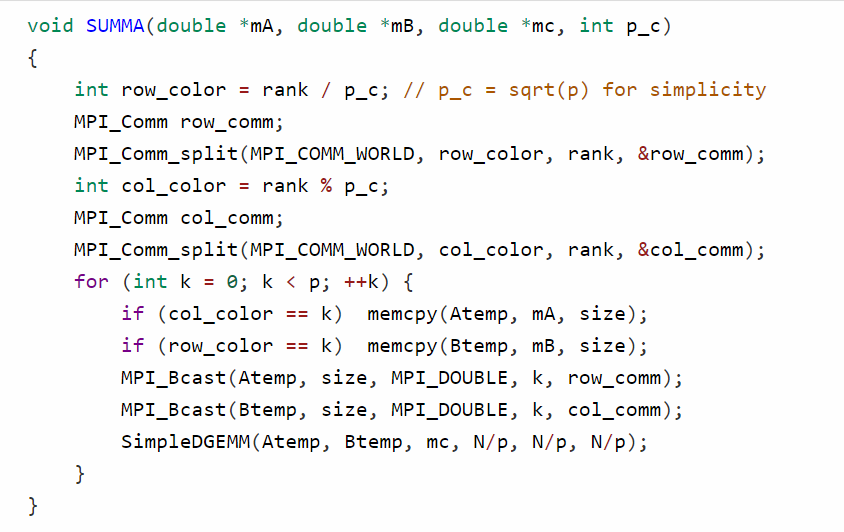
\includegraphics[width=5in]{mpi-summa.png}
%\caption{example}
\end{figure}

Ans:%upload your photo and insert it

\begin{figure}[ht]
\centering

\includegraphics[width=5in]{example.png}
%\caption{example}
\end{figure}
~\\

\bibliographystyle{plain}
\end{document}
